Throughout this course, a column vector
\[
    \begin{pmatrix}
        a \\ b \\ c
    \end{pmatrix}
\]
is interpreted as the vector $ \mathbf{x} = a \mathbf{e}_x+b \mathbf{e}_y+ c \mathbf{e}_z $ where $ \mathbf{e}_i $ are basis vectors aligned with the \textit{fixed} Cartesian $x$-$y$-$z$ axes in $ \mathbb{R}^{3} $.
\section{Differential Geometry of Curves}
\subsection{Parametrised curves and arc lengths}

\begin{definition}[Parametrised curve]
    A \textbf{parametrised curve} in $ \mathbb{R}^{3} $ is the image of a continuous map $ \mathbf{x}: [a,b]\to \mathbb{R}^{3} $ where $ t \to \mathbf{x}(t) $. In Cartesian coordinates,
    \[
        \mathbf{x}(t)=\begin{pmatrix}
            x_1(t) \\ x_2(t) \\ x_3(t)
        \end{pmatrix} = \begin{pmatrix}
            x(t) \\ y(t) \\ z(t)
        \end{pmatrix}.
    \]
\end{definition}
\begin{definition}[Differentialble, regular, and smooth curves]
    We say $C$ is a \textbf{differentiable} if each of the components $ \{x_i(t)\}_{i=1}^3 $ are differentiable. It is \textbf{regular} if $ |\mathbf{x}'(t)|\neq 0 $. If $C$ is differentiable and regular, then we say $C$ is \textbf{smooth}.
\end{definition}
\begin{note}
    The regular condition \textit{is} needed. Consider $ \mathbf{x}(t)=(t^2,t^3) $, then $ \mathbf{x} $ is differentiable but has a cusp at $t=0$, that $ \mathbf{x}'(0)=0 $.
\end{note}
Recall that $x_i(t)$ is differentiable at $t$ if
\[
    x_i(t+h) = x_i(t) + x_i'(t) h+o(h).
\]
\begin{definition}[Vector definition of derivatives]
    The derivative $ \mathbf{x}'(t) $ is defined as
    \[
        \mathbf{x}(t+h) = \mathbf{x}(t) + \mathbf{x}'(t)h + o(h),
    \]
    where $o(h)$ is a vector for which $ |o(h)|/h\to 0 $.
\end{definition}
\subsubsection*{Finding lengths}

Approximate $C$ using straight lines. Introduce a \textit{partition} $P$ of $[a,b]$ that $ t_0 = a, t_N = b $,
\[
    t_0<t_1<\cdots<t_N.
\]
Set $ \Delta t_i = t_{i+1}-t_i $ and $ \Delta t = \max_i \Delta t_i $.
\begin{definition}[Relative length]
    Define length of $C$ \textit{relative} to $P$ by
    \[
        \ell (C,P) = \sum_{i=0}^{N-1} \left| \mathbf{x}(t_{i+1})-\mathbf{x}(t_i) \right|.
    \]
\end{definition}

\begin{center}
\begin{tikzpicture}
    \draw[color=blue] plot [smooth, tension=1] coordinates {(0,0) (3,1) (6,-1.2) (8,0)};
    \draw[->-=0.5, color=red] (0,0) -- (3,1);
    \draw[->-=0.5, color=red]  (6,-1.2) -- (8,0);
    \draw[->-=0.5, color=red]  (3,1) -- (6,-1.2);
\end{tikzpicture}
\end{center}

\begin{definition}[Length of curve, rectifiability]
    Define \textbf{length} of $C$ by
    \[
        \ell (C) = \lim_{\Delta t \to 0} \ell (C,P).
    \]
    If the limit does not exist, $C$ is said to be \textbf{non-rectifiable}.
\end{definition}

Suppose $C$ is differentiable. Then
\begin{align*}
    \mathbf{x}(t_{i+1}) & = \mathbf{x}(t_i+t_{i+1}-t_i)                                   \\
                        & = \mathbf{x}(t_i+ \Delta t_i)                                   \\
                        & = \mathbf{x}(t_i) + \mathbf{x}'(t_i)\Delta t_i + o(\Delta t_i).
\end{align*}
It follows that
\[
    \left| \mathbf{x}(t_{i+1})- \mathbf{x}(t_i)\right| =\left| \mathbf{x}'(t_i) \right| \Delta t_i + o(\Delta t_i),
\]
and thus 
\[
    \ell (C,P) = \sum_{i=0}^{N-1} \left| \mathbf{x}'(t_i) \right| \Delta t_i + o(\Delta t_i).
\]
Therefore for any $ \epsilon>0 $, if $ \Delta t $ is \textit{sufficiently} small, we have 
\[
    \left| o(\Delta t_i) \right| < \frac{\epsilon }{b-a} \Delta t_i, \quad i=0,\dots,N-1.
\]
So 
\begin{align*}
    \left| \ell (C,P) - \sum_{i=0}^{N-1} \left| \mathbf{x}'(t_i) \right| \Delta t_i \right| &= \left| \sum_{i=0}^{N-1} o(\Delta t_i) \right| \\ 
    &< \frac{\epsilon}{b-a} \sum_{i=0}^{N-1} \Delta t_i = \epsilon.
\end{align*}

\begin{definition}[Detailed definition of lengths]
    The length of $C$ can be computed explicitly as 
    \[
        \ell (C) = \lim_{\Delta t \to 0} \sum_{i=0}^{N-1} \left| \mathbf{x}'(t_i) \right| \Delta t_i = \int_{a}^{b} \left| \mathbf{x}'(t) \right|  \,\mathrm{d}t.
    \]
    See Analysis I for Riemann integrals. We write 
    \[
        \ell (C) = \int_{C} \,\mathrm{d}s,
    \]
    where $ \rmd s $ is called the \textbf{arc-length element}, so $ \rmd s = |\mathbf{x}'(t)| \dd t $.
\end{definition}
\begin{definition}[Line integral]
    The \textbf{line intergal} of $f(\bfx)$ along $C$ is defined by 
    \[
        \int_{C} f(\mathbf{x}) \,\mathrm{d}s = \int_{a}^{b} f(\mathbf{x}(t)) \left| \bfx'(t) \right| \,\mathrm{d}t.
    \]
\end{definition}
\begin{definition}[Piecewise smooth curve]
    Call $C$ \textbf{piecewise smooth} if $C$ is made up of $M$ smooth curves $ C_1,\dots,C_M $. Write $C=C_1+\cdots+C_M$ and the line integral along $C$ is defined as 
    \[
        \int_{C} f(\mathbf{x}) \,\mathrm{d}s = \sum_{i=1}^{M}\int_{C_i} f(\mathbf{x}) \,\mathrm{d}s.
    \]
\end{definition}
\begin{note}
    (Informally) 
    \[
        \rmd s = |\mathbf{x}'(t)|\dd t = \sqrt{\left( \frac{\mathrm{d}x}{\mathrm{d}t}  \right)^2+\left(\frac{\mathrm{d}y}{\mathrm{d}t}  \right)^2+\left(\frac{\mathrm{d}z}{\mathrm{d}t}  \right)^2}\dd t,
    \]
    i.e.
    \[
        \rmd s^2 = \rmd x^2+\rmd y^2+\rmd z^2.
    \]
    This is known as the Pythagorean theorem.
\end{note}
\begin{example}
    Let $C$ be a circle of radius $r$. Reproduce the process to find the curve length of $C$, i.e. the parameter. Check that 
    \[
        \int_{C} x^2y \,\mathrm{d}s = 0.
    \]
\end{example}

\subsubsection*{Change of parametrisations}

Suppose $C$ has 2 different parametrisations
\begin{align*}
    \mathbf{x} &= \mathbf{x}_1(t), \quad a\le t\le b,\\
    \mathbf{x} &= \mathbf{x}_2(\tau),\quad \alpha\le \tau\le \beta.
\end{align*}
We must have $ \bfx_2(\tau) = \bfx_1(t(\tau)) $ for some function $t(\tau)$. Assume that $ \frac{\mathrm{d}t}{\mathrm{d}\tau}\neq 0  $, so that $ t(\tau) $ is invertible and differentiable(see inverse function theorem in Analysis and Topology). Note that 
\begin{align*}
    \frac{\mathrm{d}}{\mathrm{d}\tau} \mathbf{x}_2(\tau) &= \frac{\mathrm{d}}{\mathrm{d}\tau} \mathbf{x}_1(t(\tau))\\
    &= \bfx_1'(t(\tau)) \frac{\mathrm{d}t}{\mathrm{d}\tau}.  
\end{align*}
Hence we can make the substitution $ t=t(\tau) $. Assume that $ \frac{\mathrm{d}t}{\mathrm{d}\tau}>0  $, then 
\[
    \int_{a}^{b} f(\bfx_1(t)) |\mathbf{x}_1'(t)| \,\mathrm{d}t = \int_{\alpha}^{\beta} f(\bfx_2(\tau))|\mathbf{x}_1'(t(\tau))| \frac{\mathrm{d}t}{\mathrm{d}\tau}  \,\mathrm{d}\tau = \int_{\alpha}^{\beta} f(\bfx_2(\tau))|\mathbf{x}_2'(\tau)| \,\mathrm{d}\tau.
\]
Similarly it holds for $ \frac{\mathrm{d}t}{\mathrm{d}\tau}<0  $. Hence
\begin{proposition}\label{prop:change of parametrisations}
    $ \displaystyle \int_{C} f(\bfx) \,\mathrm{d}s $ is \textit{invariant} under different parametrisations.
\end{proposition}

\subsubsection*{Parametrisation by arc-length}
Note that we can parametrise curves in various ways. Define \textbf{arc-length} function for curve $ [a,b]\ni t \mapsto \mathbf{x}(t) $ by 
\[
    s(t) = \int_{a}^{t} \left| \bfx'(\tau) \right| \,\mathrm{d}\tau,
\]
so that $s(a)=0$ and $ s(b)=\ell (C) $. Also 
\[
    \frac{\mathrm{d}s}{\mathrm{d}t} = \left| \bfx'(t) \right| \ge 0, 
\]
so for regular curves we have $ \rmd s/\rmd t >0 $, and we can revert relationship between $s$ and $t$ to find $t=t(s)$. So we can parametrise \textit{regular} curves with respect to arc-length. Write $ \mathbf{r}(s)=\mathbf{x}(t(s)) $ where $ 0\le s\le \ell (C) $, then by chain rule, 
\[
    \frac{\mathrm{d}t}{\mathrm{d}s} = \frac{1}{\rmd s/\rmd t} = \frac{1}{\left| \mathbf{x}'(t(s)) \right| }
\]
and 
\begin{align*}
    \mathbf{r}'(s)&= \frac{\mathrm{d}}{\mathrm{d}s}\mathbf{x}(t(s))=\frac{\mathrm{d}t}{\mathrm{d}s}\mathbf{x}'(t(s))\\ 
    &= \frac{\mathbf{x}'(t(s))}{\left| \mathbf{x}'(t(s)) \right|} \Longrightarrow \left| \bfr'(s) \right| =1. \\ 
\end{align*}
This gives 
\[
    \ell (C) = \int_{0}^{\ell (C)} \left| \bfr'(s) \right| \,\mathrm{d}s = \int_{0}^{\ell (C)} \,\mathrm{d}s
\]

\subsection{Curvature and torsion}
Throughout this subsection we talk about generic \textit{regular curves} $C$ parametrised by \textit{arc-length} and write as $ s \mapsto \mathbf{r}(s) $. Define \textbf{tangent vector} $ \bft(s)=\mathbf{r}'(s) $, then $ |\bft(s)|=1 $. Since $ |\bft(s)| $ does not change, $ \bfr''(s)=\bft'(s) $ only measures change in \textit{direction}.

\begin{definition}[Curvature]
    The \textbf{curvature} of a curve $C$ at $s$ is 
    \[
        \kappa(s) = \left| \bfr''(s) \right| = \left| \bft'(s) \right|.
    \]
\end{definition}

Note that $ (\bft \cdot \bft =1)' \Rightarrow \bft \cdot \bft'=0 $.
\begin{definition}[Principal normal]
    The \textbf{principal normal} $\bfn$ is defined by 
    \[
        \bft'=\kappa \bfn.
    \]
    Note that $ \bft \cdot \bfn=0 $ so $\bfn$ normal to $C$.
\end{definition}

\begin{definition}[Binormal]
    The \textbf{binormal} is defined as 
    \[
        \bfb = \bft \times \bfn.
    \]
\end{definition}

$ \{\bft,\bfn,\bfb\} $ is an orthonormal basis for $ \mathbb{R}^{3} $. Note that $ \bfb' \cdot \bfb=0 $ and $ \bft \cdot \bfb'=0 $\footnote{Verify this.}, so $ \bfb' \perp \bfb,\bft $ so $ \bfb' \parallel \bfn $.

\begin{definition}[Torsion]
    Define \textbf{torsion} $ \tau $ by $ \bfb' = -\tau \bfn $.
\end{definition}

\begin{proposition}
    The curvature $ \kappa(s) $ and torsion $ \tau(s)$ define a curve up to translation and/or orientation.
\end{proposition}
\begin{proof}
    Note that
    \[
        \bft'=\kappa (\bfb\times \bft)\quad \text{and}\quad \bfb'=-\tau(\bfb\times \bft).
    \]
    This is 6 equations for 6 unknowns. Hence given $ \kappa(s),\tau(s),\bft(0),\bfb(0) $ can construct $ \bft(s),\bfb(s) $ and hence $\bfn=\bfb\times \bft$. Hence the result.
\end{proof}

\subsection{Radius of curvature}
Taylor expand $ \mathbf{r}(s) $ about $s=0$(write $ \bft=\bft(0) $, etc.):
\begin{align*}
    \bfr(s)&= \mathbf{r}(0)+s \mathbf{r}'(0)+\frac{1}{2}s^2 \bfr''(0)+o(s^2)\\
    &= \mathbf{r}+s\bft+\frac{1}{2}s^2 \kappa \bfn + o(s^2).\tag{$*$}\label{eq:1.3.1}
\end{align*}

Suppose wlog that $\bft$ is horizontal. What cirle that goes through the curve \textit{tangentially} at $ \bfr=\bfr(0) $ is \textit{best fit}?
\begin{center}
    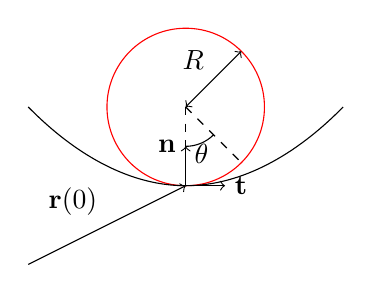
\begin{tikzpicture}
      \draw[color=red] circle [radius = 1];
      \draw [<->] (0, 0) -- (0.707, 0.707) node [anchor = south east, pos = 0.5] {$R$};
      \draw [->] (-2, -2) -- (0, -1) node [anchor = south east, pos = 0.5] {$\mathbf{r}(0)$};
      \draw [->] (0, -1) -- (0.5, -1) node [right] {$\mathbf{t}$};
      \draw [->] (0, -1) -- (0, -0.5) node [left] {$\mathbf{n}$};
      \draw [dashed] (0, 0) -- (0, -1);
      \draw [dashed] (0, 0) -- (0.707, -0.707);
      \draw (0, -0.5) arc (270:315:0.5);
      \node at (0.2, -0.6) {$\theta$};
      \draw (-2, 0) parabola bend (0, -1) (2, 0);
    \end{tikzpicture}
\end{center}
The equation of the circle is given by
\[
    \mathbf{x}(\theta) = \mathbf{r} + R(1-\cos \theta)\bfn+R \sin \theta \bft.\footnote{Verify this.}
\]
Expand for $ |\theta| $ small:
\[
    \mathbf{x}(\theta) = \mathbf{r}+R \theta\bft+\frac{1}{2}R\theta^2 \bfn+o(\theta^2).
\]
Arc length on the circle is $ s=R\theta $:
\[
    \mathbf{x}(\theta)=\mathbf{r}+s\bft+\frac{1}{2R}s^2\bfn+o(s^2).
\]
Hence to match with (\ref{eq:1.3.1}) up to 2nd order, we need
\[
    R=\frac{1}{\kappa}.
\]

\begin{definition}[Radius of curvature]
    The \textbf{radius of curvature} is defined as 
    \[
        R(s)=\frac{1}{\kappa(s)}.
    \]
\end{definition}

\subsection{Gaussian curvature}

\begin{definition}[Gaussian curvature]
    Consider a surface $S$. The \textbf{Gaussian curvature} $ \kappa_G $ is defined by 
    \[
        \kappa_G=\kappa_{\text{min}}\cdot \kappa_{\text{max}},
    \]
    where $ \kappa_{\text{min}} $ and $ \kappa_{\text{max}} $ are the minimum and maximum curvatures of the curves obtained by intersecting the surface with a plane containing the normal of the surface.
\end{definition}

\begin{example}
    The Gaussian curvatrue of a plane is 0.
\end{example}
\begin{example}
    The Gaussian curvature of a sphere with radius $R$ is $ 1/R^2 $.
\end{example}

\begin{theorem}[Gauss]\label{thm:Gauss}
    Gaussian curvature of surface $S$ is invariant if you bend the surface without streching it.
\end{theorem}